% !TeX program = xelatex
\documentclass[12pt,a4paper]{ctexart}

% ============ 中文支持与字体 ============
\usepackage{ctex}
\setCJKmainfont{SimSun}[AutoFakeBold=3]
\setCJKsansfont{KaiTi}
\setCJKmonofont{SimHei}

% ============ 页面布局 ============
\usepackage[top=2.5cm, bottom=2.5cm, left=2.8cm, right=2.8cm]{geometry}

% ============ 颜色与图形 ============
\usepackage[dvipsnames,svgnames]{xcolor}
\usepackage{tikz}
\usetikzlibrary{shapes.geometric, arrows, positioning, fit, backgrounds, shadows, arrows.meta, calc, decorations.pathreplacing}
\usepackage{tcolorbox}
\tcbuselibrary{skins, breakable}

% ============ 数学与算法 ============
\usepackage{amsmath, amssymb, amsthm}
\usepackage{mathtools}

% ============ 代码与列表 ============
\usepackage{listings}
\usepackage{enumitem}

% ============ 表格 ============
\usepackage{booktabs, tabularx, multirow}

% ============ 超链接与书签 ============
\usepackage{hyperref}
\hypersetup{
  colorlinks=true,
  linkcolor=NavyBlue,
  urlcolor=RoyalBlue,
  citecolor=ForestGreen,
  pdftitle={编译器导论 — Chapter 1 讲解},
  pdfauthor={Lecture Notes},
  pdfsubject={Introduction to Compilers},
  pdflang={zh-CN},
  bookmarksnumbered=true,
  bookmarksopen=true
}

% ============ 自定义颜色 ============
\definecolor{mainblue}{HTML}{2B579A}
\definecolor{subblue}{HTML}{3A7BD5}
\definecolor{lightblue}{HTML}{E8F0FE}
\definecolor{accent}{HTML}{E74C3C}
\definecolor{codebg}{HTML}{F5F5F5}
\definecolor{notebg}{HTML}{FFF8E1}
\definecolor{warnbg}{HTML}{FFEBEE}

% ============ 自定义盒子样式 ============
\newtcolorbox{keybox}{
  colback=lightblue, colframe=mainblue, sharp corners, boxrule=0.5mm,
  fonttitle=\bfseries\sffamily, title=\textbf{核心概念}
}

\newtcolorbox{notebox}{
  colback=notebg, colframe=orange!60!yellow, sharp corners, boxrule=0.3mm,
  fonttitle=\bfseries, title=\textbf{📝 笔记}
}

\newtcolorbox{warnbox}{
  colback=warnbg, colframe=accent, sharp corners, boxrule=0.4mm,
  fonttitle=\bfseries, title=\textbf{⚠ 注意事项}
}

% ============ 自定义命令 ============
\newcommand{\compiler}{编译器\ }
\newcommand{\Compiler}{编译器\ }
\newcommand{\ir}{IR\ }
\newcommand{\IR}{IR\ }
\newcommand{\astt}{AST\ }
\newcommand{\AST}{AST\ }
\newcommand{\lexer}{词法分析器\ }
\newcommand{\parser}{语法分析器\ }

% 术语标注
\newcommand{\term}[1]{\textbf{\textcolor{mainblue}{#1}}}
\newcommand{\enterm}[1]{\textbf{\textcolor{subblue}{#1}}}

% 章节标题样式
\usepackage{titlesec}
\titleformat{\section}
  {\normalfont\LARGE\bfseries\color{mainblue}}
  {\thesection}{1em}{}
\titleformat{\subsection}
  {\normalfont\Large\bfseries\color{subblue}}
  {\thesubsection}{1em}{}
\titleformat{\subsubsection}
  {\normalfont\large\bfseries}
  {\thesubsubsection}{1em}{}

% ============ 代码样式 ============
\lstset{
  basicstyle=\ttfamily\small,
  backgroundcolor=\color{codebg},
  frame=single,
  framerule=0.3mm,
  rulecolor=\color{gray!50},
  tabsize=2,
  breaklines=true,
  xleftmargin=1em,
  xrightmargin=1em
}

% ============ 文档信息 ============
\title{
  \vspace{2cm}
  {\Huge\bfseries\color{mainblue} 编译器导论}\\[0.5cm]
  {\Large\color{subblue} Chapter 1: Introduction to Compilers}\\[1cm]
  {\normalsize\color{gray} 基于南京大学计算机学院课程讲义}\\[0.3cm]
  {\normalsize\color{gray} 时清凯 \texttt{|} qingkaishi@nju.edu.cn}
  \vspace{1cm}
}
\author{}
\date{\today}

\begin{document}

\maketitle
\thispagestyle{empty}

% ==================== 目录 ====================
\newpage
\setcounter{page}{1}
\tableofcontents
\newpage

% ==================== 前言 ====================
\section*{前言}
\addcontentsline{toc}{section}{前言}

本文是对《编译器导论》课程第一章 $\langle$Introduction to Compilers$\rangle$ 的详细讲解笔记。原始讲义由南京大学计算机学院时清凯老师制作，共包含 131 页幻灯片。本文将其内容重新组织为四个主要部分，并以适合阅读和学习的形式呈现：

\begin{enumerate}[leftmargin=2em, itemsep=0.3em]
  \item \textbf{第一部分：什么是编译器？} — 编译器的基本概念、编译器与解释器/链接器的区别、编译器的整体架构（前端、中端、后端）
  \item \textbf{第二部分：开发工具} — 编译器开发中使用的各类工具（词法/语法分析器生成器等）
  \item \textbf{第三部分：编译器的应用} — 编译器技术在不同领域的应用场景
  \item \textbf{第四部分：编程语言术语回顾} — 编程范型、类型系统、作用域与函数调用等基础概念
\end{enumerate}

\vspace{0.5cm}
本文适合作为学习编译器原理的入门材料，建议读者配合原始讲义 Slides 一起使用。

\newpage

% ==================== 第一部分：什么是编译器？ ====================
\section{第一部分：什么是编译器？}

\subsection{编译器的基本定义}

\begin{keybox}
  \term{编译器（Compiler）} 是一种将\emph{源语言（Source Language）} 编写的程序翻译为\emph{目标语言（Target Language）} 程序的软件工具。
\end{keybox}

典型的编译场景包括：
\begin{itemize}[itemsep=0.2em]
  \item C/C++/Java $\rightarrow$ x86 机器码 / Java Bytecode
  \item 近年来还出现了 \textbf{语言到语言的转译器（Transpiler）}，例如 C $\rightarrow$ Rust 的翻译工具
\end{itemize}

\begin{figure}[h]
\centering
\begin{tikzpicture}[
  node distance=2cm,
  box/.style={rectangle, draw=mainblue, thick, fill=lightblue, minimum width=3cm, minimum height=1cm, align=center, rounded corners},
  arrow/.style={->, >=Stealth, thick, draw=mainblue}
]
  \node[box] (src) {源程序\\(C, C++, Java...)};
  \node[box, right=of src] (compiler) {\Compiler\\};
  \node[box, right=of compiler] (tgt) {目标程序\\(x86, ARM, Bytecode...)};
  \draw[arrow] (src) -- (compiler);
  \draw[arrow] (compiler) -- (tgt);
\end{tikzpicture}
\caption{编译器：源语言 $\rightarrow$ 目标语言}
\end{figure}

\subsection{编译器 vs. 解释器 vs. 链接器}

\subsubsection{编译器与解释器的区别}

\begin{keybox}
  \term{解释器（Interpreter）} 不将源程序翻译为另一种语言，而是\emph{直接解释并执行}源语言中的语句。
\end{keybox}

\begin{table}[h]
\centering
\begin{tabularx}{\textwidth}{@{}lXX@{}}
\toprule
\textbf{特性} & \textbf{编译器} & \textbf{解释器} \\
\midrule
工作方式 & 先将整个程序翻译为目标代码，再执行 & 逐条读取源程序语句，直接执行 \\
输出产物 & 生成独立的目标程序文件 & 不产生独立的可执行文件 \\
执行效率 & 高（一次翻译，多次执行） & 低（每次执行都需要解析） \\
典型语言 & C, C++, Rust, Go & Python, Shell, JavaScript \\
\bottomrule
\end{tabularx}
\caption{编译器与解释器的对比}
\end{table}

\begin{notebox}
  \textbf{Java 是一个特殊案例：} Java 使用了 \textbf{编译器 + 解释器 + JIT（Just-In-Time）编译器} 的组合策略：
  \begin{enumerate}
    \item 首先由 \texttt{javac} 编译器将 Java 源码编译为字节码（Bytecode）
    \item 运行时由 JVM 的解释器逐条解释字节码
    \item JIT 编译器将热点代码（Hotspot）编译为本地机器码以提高性能
  \end{enumerate}
\end{notebox}

\subsubsection{编译器与链接器的关系}

\begin{keybox}
  \term{链接器（Linker）} 将多个编译单元（Compilation Units）链接为单个文件，可以是可执行文件（Executable）、静态库（Static Library）或动态库（Dynamic Library）。
\end{keybox}

以 GCC 为例说明编译与链接的完整流程：

\begin{figure}[h]
\centering
\begin{tikzpicture}[
  node distance=1.5cm,
  file/.style={rectangle, draw=gray, thick, fill=codebg, minimum width=2cm, minimum height=0.7cm, align=center, rounded corners},
  process/.style={rectangle, draw=mainblue, thick, fill=lightblue, minimum width=2cm, minimum height=0.7cm, align=center, rounded corners},
  arrow/.style={->, >=Stealth, thick}
]
  \node[file] (f1) {file1.c};
  \node[file, right=1.5cm of f1] (f2) {file2.c};
  \node[file, right=1.5cm of f2] (f3) {file3.c};

  \node[process, below=1cm of $(f1)!0.5!(f2)$] (compile) {编译 (Compile)\\\texttt{gcc -c}};

  \node[file, below=1cm of f1 |- compile] (o1) {file1.o};
  \node[file, below=1cm of f2 |- compile] (o2) {file2.o};
  \node[file, below=1cm of f3 |- compile] (o3) {file3.o};

  \node[process, below=1cm of $(o1)!0.5!(o3)$] (link) {链接 (Link)\\\texttt{gcc *.o -o exe}};

  \node[file, below=1cm of link] (exe) {executable.exe};

  \draw[arrow] (f1) -- (compile);
  \draw[arrow] (f2) -- (compile);
  \draw[arrow] (f3) -- (compile);
  \draw[arrow] (o1) -- (link);
  \draw[arrow] (o2) -- (link);
  \draw[arrow] (o3) -- (link);
  \draw[arrow] (link) -- (exe);
\end{tikzpicture}
\caption{GCC 的编译与链接流程}
\end{figure}

\subsubsection{链接的关键作用}

\begin{notebox}
  链接器的核心作用是\emph{符号解析（Symbol Resolution）}。例如：
  \begin{itemize}
    \item \texttt{file1.c} 中 \textbf{声明} 并 \textbf{调用} 了函数 \texttt{foo()}
    \item \texttt{file2.c} 中 \textbf{定义}（实现）了函数 \texttt{foo()}
  \end{itemize}
  编译阶段，\texttt{file1.o} 中会记录一个对 \texttt{foo} 的\emph{未解析引用}；在链接阶段，链接器会将其与 \texttt{file2.o} 中 \texttt{foo} 的定义\emph{绑定（bind）}起来。

  此外，链接器还能链接第三方库（\texttt{-lxxx} 选项）。
\end{notebox}

\subsection{编译器的工作流程：三阶段架构}

编译器通常分为\emph{前端（Front End）}、\emph{中端（Middle End）} 和\emph{后端（Back End）} 三个阶段。

\begin{figure}[h]
\centering
\begin{tikzpicture}[
  node distance=1.5cm,
  phase/.style={rectangle, draw=accent, thick, fill=warnbg, minimum width=3.5cm, minimum height=1.2cm, align=center, rounded corners, font=\bfseries},
  sub/.style={rectangle, draw=mainblue, thick, fill=lightblue, minimum width=2.5cm, minimum height=0.8cm, align=center, rounded corners, font=\small},
  arrow/.style={->, >=Stealth, thick}
]
  \node[phase] (front) {前端 (Front End)};
  \node[phase, right=1.5cm of front] (middle) {中端 (Middle End)};
  \node[phase, right=1.5cm of middle] (back) {后端 (Back End)};

  \node[sub, below=0.5cm of front] (fdetail) {源程序 $\rightarrow$ IR\\词法/语法/语义分析};
  \node[sub, below=0.5cm of middle] (mdetail) {IR $\rightarrow$ IR\\机器无关优化};
  \node[sub, below=0.5cm of back] (bdetail) {IR $\rightarrow$ 目标代码\\机器相关优化};

  \draw[arrow] (front) -- (middle) node[midway, above] {IR};
  \draw[arrow] (middle) -- (back) node[midway, above] {IR};
\end{tikzpicture}
\caption{编译器的三阶段架构}
\end{figure}

\subsubsection{前端（Front End）}

前端负责读取源文件中的文本，并将其翻译为\emph{中间表示（Intermediate Representation, IR）}。主要步骤包括：

\begin{enumerate}[itemsep=0.3em]
  \item \textbf{词法分析（Lexical Analysis）}：将字符流转换为 Token 流
  \item \textbf{语法分析（Syntax Analysis）}：根据 Token 流构建抽象语法树（AST）
  \item \textbf{语义分析（Semantic Analysis）}：检查程序的语义正确性，装饰 AST
  \item \textbf{IR 生成（IR Generation）}：基于语法树生成机器无关的中间表示（如三地址码）
\end{enumerate}

\subsubsection{中端（Middle End）}

中端在 IR 上执行\emph{机器无关的优化（Machine-Independent Optimizations）}。优化的优势在于：

\begin{itemize}
  \item 相比在源码上优化：IR 提供了\emph{标准化的形式}，更易于处理
  \item 相比在机器码上优化：IR 提供了\emph{机器无关的抽象}，并保留了源码信息（如通过符号表获取类型信息）
\end{itemize}

\subsubsection{后端（Back End）}

后端负责将 IR 翻译为目标机器代码，并执行\emph{机器相关的优化}。主要步骤包括：

\begin{enumerate}[itemsep=0.3em]
  \item \textbf{指令选择（Instruction Selection）}：将 IR 映射为目标机器的指令
  \item \textbf{寄存器分配（Register Allocation）}：将变量映射到物理寄存器
  \item \textbf{指令调度（Instruction Scheduling）}：重排指令顺序以利用指令级并行
\end{enumerate}

\newpage

% ==================== 编译流程详解 ====================
\section{编译流程详解}

本节深入编译器前端的各个步骤，以具体示例展示编译过程的每一个环节。

\subsection{词法分析（Lexical Analysis）}

\begin{keybox}
  \term{词法分析} 的任务是：根据\emph{模式（Pattern）} 找到\emph{词素（Lexeme）}，并创建对应的\emph{Token}。
\end{keybox}

\textbf{三个核心概念：}
\begin{itemize}[itemsep=0.2em]
  \item \enterm{Lexeme（词素）}：源代码中的一个字符序列（字符串）
  \item \enterm{Pattern（模式）}：匹配词素的正则表达式规则；如果没有任何模式匹配，则产生词法错误
  \item \enterm{Token（词法单元）}：$\langle\text{token-class}, \text{attribute}\rangle$ 对，其中 attribute 用于区分同一类中的不同 token
\end{itemize}

\begin{figure}[h]
\centering
\textbf{示例：} 源码片段 \texttt{position = initial + rate * 60} 的词法分析过程

\vspace{0.3em}
\begin{tikzpicture}[
  procstep/.style={rectangle, draw=mainblue, thick, fill=lightblue, minimum width=2cm, minimum height=0.7cm, align=center, rounded corners, font=\footnotesize},
  arrow/.style={->, >=Stealth, thick, draw=mainblue}
]
  \node[procstep] (s1) {原始字符流};
  \node[procstep, right=of s1] (s2) {识别词素};
  \node[procstep, right=of s2] (s3) {匹配模式};
  \node[procstep, right=of s3] (s4) {生成 Token};

  \draw[arrow] (s1) -- (s2);
  \draw[arrow] (s2) -- (s3);
  \draw[arrow] (s3) -- (s4);

  \node[below=0.5cm of s2, font=\footnotesize] {\texttt{position}};
  \node[below=0.5cm of s3, font=\footnotesize] {标识符模式};
  \node[below=0.5cm of s4, font=\footnotesize] {$\langle\text{id}, 1\rangle$};
\end{tikzpicture}
\caption{词法分析的处理流程}
\end{figure}

\textbf{词法分析结果示例：}

\begin{center}
\begin{tabular}{@{}c|c|c@{}}
\toprule
\textbf{词素（Lexeme）} & \textbf{Token 类} & \textbf{属性值} \\
\midrule
\texttt{position} & id  & 1（符号表入口）\\
\texttt{=}        & =   & — \\
\texttt{initial}  & id  & 2（符号表入口）\\
\texttt{+}        & +   & — \\
\texttt{rate}     & id  & 3（符号表入口）\\
\texttt{*}        & *   & — \\
\texttt{60}       & number & 60 \\
\bottomrule
\end{tabular}
\end{center}

\begin{warnbox}
  词法分析过程中，如果遇到任何无法匹配任何模式的字符序列，将产生\emph{词法错误（Lexical Error）}。
\end{warnbox}

\subsection{语法分析（Syntax Analysis）}

\begin{keybox}
  \term{语法分析} 的任务是：接收词法分析产生的 Token 流，根据语言的文法规则，构建\emph{抽象语法树（Abstract Syntax Tree, AST）}。
\end{keybox}

\textbf{对上述 Token 流构建的 AST：}

\begin{figure}[h]
\centering
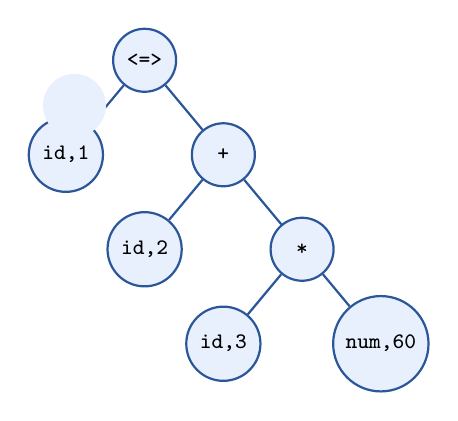
\begin{tikzpicture}[
  level distance=1.2cm,
  sibling distance=2cm,
  every node/.style={circle, draw=mainblue, thick, fill=lightblue, minimum size=0.8cm, font=\footnotesize\ttfamily},
  edge from parent/.style={draw=mainblue, thick}
]
\node {<=>}
  child { node (id1) {id,1}
    edge from parent node[left, draw=none, font=\footnotesize] {}
  }
  child { node {+}
    child { node (id2) {id,2} }
    child { node {*}
      child { node (id3) {id,3} }
      child { node {num,60} }
    }
  };
\end{tikzpicture}
\caption{\texttt{position = initial + rate * 60} 的抽象语法树}
\label{fig:ast}
\end{figure}

\noindent AST 反映了表达式的运算优先级（乘法优先于加法，赋值优先级最低）。

\subsection{语义分析（Semantic Analysis）}

\begin{keybox}
  \term{语义分析} 检查程序的\emph{语义正确性}，并为 AST 添加\emph{语义装饰（Semantic Decoration）}，如类型信息、作用域信息等。
\end{keybox}

\begin{warnbox}
  \textbf{通过语法分析并不意味着程序是正确的！} 例如以下情况语法上合法但语义错误：
  \begin{itemize}
    \item 类型不匹配（将浮点数赋给期望整数的地方）
    \item 使用未声明的变量
    \item 重复声明变量
  \end{itemize}
\end{warnbox}

在语义分析中，编译器会利用符号表（Symbol Table）为 AST 节点标注类型信息：

\begin{figure}[h]
\centering
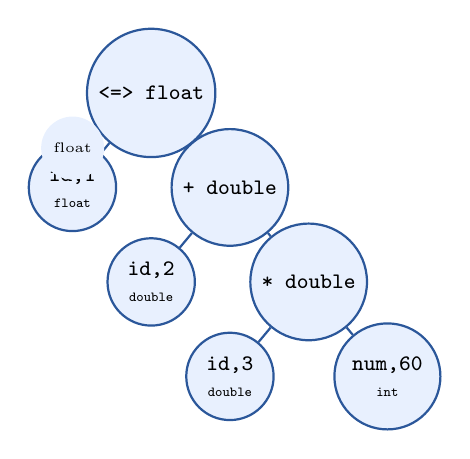
\begin{tikzpicture}[
  level distance=1.2cm,
  sibling distance=2cm,
  every node/.style={circle, draw=mainblue, thick, fill=lightblue, minimum size=0.8cm, font=\footnotesize\ttfamily, align=center},
  edge from parent/.style={draw=mainblue, thick}
]
\node {<=> float}
  child { node (id1) {id,1\\\tiny float}
    edge from parent node[left, draw=none, font=\tiny] {float}
  }
  child { node {+ double}
    child { node (id2) {id,2\\\tiny double} }
    child { node {* double}
      child { node (id3) {id,3\\\tiny double} }
      child { node {num,60\\\tiny int} }
    }
  };
\end{tikzpicture}
\caption{添加类型信息后的 AST}
\end{figure}

语义分析过程中，编译器会进行类型检查：例如 \texttt{float = double} 的隐式转换是否合法？若不合法的隐式转换发生，应产生\emph{警告或错误}。

\subsection{IR 生成（Intermediate Code Generation）}

\begin{keybox}
  \term{中间代码生成} 基于 AST 生成\emph{机器无关的中间表示（IR）}，最常用的形式之一是\emph{三地址码（Three-Address Code）}。
\end{keybox}

以图~\ref{fig:ast} 中的 AST 为例，生成的三地址码如下：

\begin{lstlisting}[language=C, caption={三地址码示例}]
t1 = id3 * 60      // rate * 60
t2 = id2 + t1      // initial + t1
id1 = t2           // position = t2
\end{lstlisting}

三地址码的特点：
\begin{itemize}
  \item 每条指令最多包含\emph{三个操作数}（两个源操作数 + 一个目标操作数）
  \item 使用\emph{临时变量}（如 \texttt{t1, t2}）保存中间结果
  \item 形式统一，便于后续优化
\end{itemize}

\newpage

% ==================== 中端优化 ====================
\section{中端优化}

\subsection{机器无关优化的特点}

\begin{keybox}
  中端优化在 IR 上执行，是\emph{机器无关的（Machine-Independent）}。这意味着优化不依赖于特定的硬件架构。
\end{keybox}

\textbf{为什么选择在 IR 层做优化？}

\begin{enumerate}[itemsep=0.3em]
  \item \textbf{相对于源代码层面}：IR 提供了\emph{标准化的形式}，每种语言的前端都生成统一的 IR，因此优化算法可以复用
  \item \textbf{相对于机器代码层面}：IR 保留了程序的高层信息（如类型信息、控制流结构），这些在机器代码中可能已经丢失
  \item IR 抽象掉了与具体机器相关的细节，但保留了足够多的语义信息
\end{enumerate}

\subsection{优化示例}

以前面的三地址码为例，中端可以进行优化：

\begin{minipage}{0.48\textwidth}
\textbf{优化前：}
\begin{lstlisting}
t1 = id3 * 60
t2 = id2 + t1
id1 = t2
\end{lstlisting}
\end{minipage}
\hfill
\begin{minipage}{0.48\textwidth}
\textbf{优化后：}
\begin{lstlisting}
t1 = id3 * 60
id1 = id2 + t1
\end{lstlisting}
\end{minipage}

\vspace{0.3em}
这里的优化是\emph{复写传播（Copy Propagation）} +\emph{死代码消除（Dead Code Elimination）}：发现 \texttt{t2} 仅仅是将 \texttt{id2 + t1} 的值转发给 \texttt{id1}，因此可以直接将 \texttt{id2 + t1} 赋给 \texttt{id1}，并删除 \texttt{t2}。

\newpage

% ==================== 后端 ====================
\section{后端：从 IR 到目标代码}

后端负责将 IR 转换为目标机器代码，主要包含三个关键步骤。

\subsection{指令选择（Instruction Selection）}

\begin{keybox}
  \term{指令选择} 将 IR 中的每条操作映射为目标机器的具体指令序列，同时进行\emph{机器相关的优化}。
\end{keybox}

\textbf{示例：} 将 IR 指令 \texttt{a = a + 1} 翻译为两种不同质量的机器码：

\begin{minipage}{0.48\textwidth}
\textbf{朴素翻译（3条指令）：}
\begin{lstlisting}
LD  R0, a      // R0 = a
Add R0, R0, #1 // R0 = R0 + 1
ST  a,  R0     // a = R0
\end{lstlisting}
\end{minipage}
\hfill
\begin{minipage}{0.48\textwidth}
\textbf{优化翻译（1条指令）：}
\begin{lstlisting}
INC a          // a = a + 1
\end{lstlisting}
\end{minipage}

\vspace{0.3em}
指令选择的质量直接影响目标代码的\emph{大小}和\emph{执行速度}。

\subsection{寄存器分配（Register Allocation）}

\begin{keybox}
  \term{寄存器分配} 的目标是在寄存器数量\emph{有限}的约束下，尽可能将频繁访问的变量放在寄存器中，因为\emph{访问寄存器的速度远快于访问内存}。
\end{keybox}

\textbf{核心矛盾：}
\begin{itemize}
  \item CPU 中寄存器的数量非常有限（x86-64 仅有 16 个通用寄存器）
  \item 程序中可能存在成百上千个变量和临时值
  \item 寄存器分配器必须决定哪些值在何时占用寄存器，哪些值需要「溢出（Spill）」到内存
\end{itemize}

\subsection{指令调度（Instruction Scheduling）}

\begin{keybox}
  \term{指令调度} 通过重新排列指令的执行顺序，利用目标处理器的\emph{指令级并行（Instruction-Level Parallelism, ILP）} 能力，以提高代码执行效率。
\end{keybox}

现代处理器通常具有多条流水线（Pipeline），可以在同一时钟周期内执行多条\emph{相互独立的指令}。指令调度的任务就是重排指令顺序，使彼此独立的指令尽可能并行执行，同时保持程序的语义不变。

\newpage

% ==================== 课程结构 ====================
\section{课程结构}

\subsection{内容划分}

课程内容按照编译器的三阶段架构进行组织：

\begin{table}[h]
\centering
\begin{tabularx}{\textwidth}{@{}lX@{}}
\toprule
\textbf{部分} & \textbf{涵盖内容} \\
\midrule
\textbf{Part I — 前端} & 词法分析、语法分析、语义分析 \\
\textbf{Part II — 中端} & IR 生成、机器无关优化、数据流分析、符号执行 \\
\textbf{Part III — 后端} & 指令选择、寄存器分配、指令调度、SSA 翻译与反翻译 \\
\textbf{扩展主题} & 过程间分析、指针分析 \\
\bottomrule
\end{tabularx}
\caption{课程内容的三部分划分}
\end{table}

\subsection{实验安排}

课程配套 8 个实验（Labs），与理论内容紧密结合：

\begin{table}[h]
\centering
\begin{tabularx}{\textwidth}{@{}lX@{}}
\toprule
\textbf{实验} & \textbf{对应内容} \\
\midrule
Lab 1 & 词法分析 \\
Lab 2 & 语法分析 \\
Lab 3 & 语义分析 \\
Labs 4–5 & 中端优化 \\
Lab 6 & IR 生成 \\
Labs 7–8 & 后端 \\
\bottomrule
\end{tabularx}
\caption{课程实验安排}
\end{table}

\subsection{课程信息}

\begin{itemize}[itemsep=0.2em]
  \item \textbf{课程主页：} \url{https://qingkaishi.github.io/Compilers.html}
  \item \textbf{QQ 群：} 1033582067
  \item \textbf{评分方案：} 作业 0\% + 实验 70\% + 期末考试 30\%
\end{itemize}

\newpage

% ==================== 第二部分：工具 ====================
\section{第二部分：编译器开发工具}

\subsection{工具概览}

编译器开发涉及多种工具，覆盖编译流程的各个阶段。讲义中展示了一个完整的编译器工具链图示。

\subsection{主要工具分类}

\begin{enumerate}[itemsep=0.3em]
  \item \textbf{词法分析器生成器（Lexer Generator）}
  \begin{itemize}
    \item 代表工具：\texttt{lex}, \texttt{flex}, ANTLR
    \item 输入：基于正则表达式的词法规则描述
    \item 输出：C/Java 等语言的词法分析器代码
  \end{itemize}

  \item \textbf{语法分析器生成器（Parser Generator）}
  \begin{itemize}
    \item 代表工具：\texttt{yacc}, \texttt{bison}, ANTLR
    \item 输入：上下文无关文法（CFG）描述
    \item 输出：语法分析器代码（LL 分析器或 LR 分析器）
  \end{itemize}

  \item \textbf{优化框架}
  \begin{itemize}
    \item LLVM：模块化的编译器基础设施，提供了 IR、优化 Pass、代码生成等功能
    \item GCC：GNU 编译器套件，包含完整的编译与优化框架
  \end{itemize}

  \item \textbf{调试与分析工具}
  \begin{itemize}
    \item 语法树可视化工具
    \item 控制流图（CFG）/数据流图（DFG）可视化
    \item 性能剖析（Profiling）工具
  \end{itemize}
\end{enumerate}

\newpage

% ==================== 第三部分：应用 ====================
\section{第三部分：编译器的应用}

\subsection{高级编程语言的实现}

编译器最直接的应用是实现编程语言。此外，编译器技术也是实现\emph{领域特定语言（Domain-Specific Language, DSL）} 的关键。DSL 是为特定领域设计的语言（如 SQL 用于数据库查询，Verilog 用于硬件描述），其编译器通常比通用语言编译器更小、更专业化。

\subsection{计算机体系结构的设计与优化}

编译器与硬件设计相互影响。处理器厂商会提供编译器后端以支持其新指令集和微架构特性；同时编译器反馈的信息也会影响下一代处理器的设计决策。

\subsection{广泛的应用领域}

\begin{itemize}[itemsep=0.2em]
  \item \textbf{人工智能（AI）：} 深度学习框架（如 TensorFlow、PyTorch）中的计算图编译与优化（XLA, Glow, TVM 等）
  \item \textbf{游戏开发：} 着色器编译器（Shader Compiler），如 HLSL/GLSL 到 GPU 指令的编译
  \item \textbf{嵌入式系统：} 针对资源受限设备的交叉编译与优化
  \item \textbf{高性能计算（HPC）：} 自动并行化、向量化编译优化
\end{itemize}

\subsection{程序翻译（Transpilation）}

源语言到源语言的翻译是近年来的研究热点。例如：将 C 代码翻译为 Rust 代码。这类工具需要对源语言和目标语言都有深刻的理解。

\subsection{软件生产力工具}

编译器技术可应用于开发辅助工具：
\begin{itemize}[itemsep=0.2em]
  \item 代码格式化工具（如 \texttt{clang-format}）
  \item 代码重构工具（基于 AST 的语义重构）
  \item 静态分析工具（代码风格检查、潜在 Bug 检测）
  \item IDE 智能提示（自动补全、跳转定义、查找引用）
\end{itemize}

\subsection{安全保证工具}

编译器技术在安全领域有广泛应用：
\begin{itemize}[itemsep=0.2em]
  \item \textbf{Bug 发现：} 基于编译器分析的静态漏洞检测（如 Coverity、Infer）
  \item \textbf{程序插桩（Instrumentation）：} 在编译时插入额外代码以监控运行时行为（如 AddressSanitizer, ThreadSanitizer）
  \item \textbf{软件防御：} 编译时地址空间布局随机化（ASLR）、栈保护（Stack Canary）、控制流完整性（CFI）等
\end{itemize}

\newpage

% ==================== 第四部分：术语回顾 ====================
\section{第四部分：编程语言术语回顾}

\subsection{声明式语言 vs. 命令式语言}

\begin{keybox}
  \term{命令式语言（Imperative）} 通过一系列指令（Commands）\textbf{描述如何做（How to do）}，程序显示的是一步步的操作过程。

  \term{声明式语言（Declarative）} 描述\emph{要做什么（What to do）}，而不显式描述执行步骤。逻辑引擎或查询引擎负责确定「怎么做」。
\end{keybox}

\begin{table}[h]
\centering
\begin{tabular}{@{}ll@{}}
\toprule
\textbf{命令式语言} & \textbf{声明式语言} \\
\midrule
C, C++, Java, Python & Lisp, SQL, Haskell, Prolog \\
\bottomrule
\end{tabular}
\caption{典型的命令式与声明式语言}
\end{table}

\subsection{函数式编程（Functional Programming）}

\begin{keybox}
  函数式编程中，程序完全由\emph{纯函数（Pure Functions）}组成，不允许修改状态或数据（没有全局变量/可变状态）。
\end{keybox}

函数式编程的核心特征：
\begin{enumerate}[itemsep=0.2em]
  \item 没有可变状态 —— 一旦创建，数据不可变（Immutable）
  \item 函数的组合（Composition）和应用是主要驱动力
  \item \emph{高阶函数（Higher-Order Functions）：} 函数可以作为参数传递给另一个函数，也可以作为返回值返回
\end{enumerate}

\begin{notebox}
  函数式编程与 SQL 查询的相似性：
  \begin{lstlisting}
SELECT SUM(CASE WHEN some_flag = 'X'
    THEN some_column
    ELSE other_column END)
FROM ...
  \end{lstlisting}
  这个 SQL 查询没有显式的循环和中间变量，而是声明式地描述了数据处理的方式 —— 这与函数式编程「描述要什么而非怎么得到」的理念一致。
\end{notebox}

\subsection{逻辑编程（Logic Programming）}

\begin{keybox}
  逻辑编程的根基在于\emph{数学逻辑}。程序由\emph{事实（Facts）}和\emph{规则（Rules）}构成，推理引擎（Inference Engine）根据事实和规则自动推导结论。
\end{keybox}

\textbf{示例（使用 Datalog 语法）：}

\begin{lstlisting}
// 事实 (Facts)
rainy("Nanjing").
rainy("Beijing").
cold("Beijing").

// 规则 (Rule): 如果一个城市既下雨又冷，则下雪
snowy(c) :- rainy(c), cold(c).

// 查询
.output snowy
\end{lstlisting}

\textbf{推理结果：} 北京满足 \texttt{rainy \&\& cold}，因此 \texttt{snowy("Beijing")} 成立；南京只有 \texttt{rainy} 但不满足 \texttt{cold}，因此不输出。

\subsection{类型系统（Type Systems）}

\subsubsection{静态类型 vs. 动态类型}

\begin{keybox}
  \term{静态类型（Static Typing）} 和 \term{动态类型（Dynamic Typing）} 的区分在于\emph{类型信息获取的时间}：
  \begin{itemize}[itemsep=0.2em]
    \item \textbf{静态类型：} 类型在\emph{编译时}确定（如 C, Java, Rust）
    \item \textbf{动态类型：} 类型在\emph{运行时}确定（如 Python, JavaScript, Ruby）
  \end{itemize}
\end{keybox}

\begin{figure}[h]
\centering
\begin{tikzpicture}[
  box/.style={rectangle, rounded corners, minimum width=3cm, minimum height=1.5cm, align=center, font=\small},
  arrow/.style={->, >=Stealth, thick}
]
  \node[box, draw=mainblue, fill=lightblue] (static) {静态类型\\编译时检查\\C, Java, Rust};
  \node[box, draw=ForestGreen, fill=green!10, right=1cm of static] (dynamic) {动态类型\\运行时检查\\Python, JS, Ruby};

  \draw[decorate, decoration={brace, mirror, amplitude=10pt}, thick, draw=gray]
    ($(static.south west)+(0,-0.8)$) -- ($(dynamic.south east)+(0,-0.8)$)
    node[midway, below=0.4cm, font=\small] {类型信息获取时间不同};
\end{tikzpicture}
\caption{静态类型与动态类型的对比}
\end{figure}

\subsubsection{强类型 vs. 弱类型}

\begin{keybox}
  \term{强类型（Strong Typing）} 和 \term{弱类型（Weak Typing）} 的区分在于\emph{类型区分的严格程度}，即语言是否允许隐式类型转换（如从字符串到数字的自动转换）。
\end{keybox}

\begin{table}[h]
\centering
\begin{tabular}{@{}ll@{}}
\toprule
\textbf{强类型} & \textbf{弱类型} \\
\midrule
Python, Java, Rust & C, JavaScript, PHP \\
\bottomrule
\end{tabular}
\caption{强类型与弱类型的典型语言}
\end{table}

\begin{warnbox}
  \textbf{常见的误解澄清：}
  \begin{itemize}
    \item \emph{静态类型 $\neq$ 强类型}。例如 C 语言是静态类型但弱类型（允许 \texttt{void*} 到任意指针的隐式转换）
    \item \emph{动态类型 $\neq$ 弱类型}。例如 Python 是动态类型但强类型（不允许字符串和数字直接相加）
  \end{itemize}
\end{warnbox}

\subsection{作用域（Scoping）}

\begin{keybox}
  \term{静态作用域（Static/Lexical Scoping）} 和 \term{动态作用域（Dynamic Scoping）} 的区别在于\emph{变量引用在何处查找}：
  \begin{itemize}[itemsep=0.2em]
    \item \textbf{静态作用域：} 变量引用的绑定在\emph{编译时}根据程序文本的嵌套结构确定（大多数现代语言采用此方式）
    \item \textbf{动态作用域：} 变量引用的绑定在\emph{运行时}根据调用栈的上下文确定
  \end{itemize}
\end{keybox}

\subsection{函数调用（Function Invocation）}

\begin{keybox}
  \term{值传递（Call by Value）} vs.\ \term{引用传递（Call by Reference）} 决定了函数参数在调用时的传递方式。
\end{keybox}

\textbf{C/C++ 中的示例对比：}

\begin{minipage}{0.48\textwidth}
\textbf{值传递（Call by Value）：}
\begin{lstlisting}[language=C]
void swap(int x, int y) {
  int t;
  t = x;
  x = y;
  y = t;
}
// a, b 不变！
\end{lstlisting}
\end{minipage}
\hfill
\begin{minipage}{0.48\textwidth}
\textbf{引用传递（Call by Reference）：}
\begin{lstlisting}[language=C++]
void swap(int &x, int &y) {
  int t;
  t = x;
  x = y;
  y = t;
}
// a, b 将被交换
\end{lstlisting}
\end{minipage}

\vspace{0.5em}
在值传递中，\texttt{x} 和 \texttt{y} 是实参的副本；在引用传递中，\texttt{x} 和 \texttt{y} 是实参的别名（Alias），对它们的修改会直接影响原始变量。

\subsection{虚函数（Virtual Functions）}

\begin{keybox}
  \term{虚函数} 是在基类中声明、可被派生类\emph{重写（Override）}的成员函数。虚函数是实现\emph{运行时多态（Runtime Polymorphism）}的机制。
\end{keybox}

\begin{itemize}[itemsep=0.2em]
  \item 在 Java 中，任何非 private、非 static、非 final 的方法都是虚函数
  \item 虚函数的调用在编译时无法确定具体调用哪个实现，需要在运行时通过\emph{虚函数表（vtable）}动态派发（Dynamic Dispatch）
\end{itemize}

\textbf{示例：}

\begin{lstlisting}[language=Java]
void add(List<Integer> list, int y) {
    list.add(y);  // 调 ArrayList.add() 还是 LinkedList.add()?
}
\end{lstlisting}

在编译时，编译器只知道 \texttt{list} 的类型是 \texttt{List} 接口，无法确定实际运行时对象是 \texttt{ArrayList} 还是 \texttt{LinkedList}。调用哪个 \texttt{add} 方法需要在运行时通过虚函数机制动态决定。

\newpage

% ==================== 总结 ====================
\section{课程总结}

本节作为编译器课程的入门章节，涵盖了以下核心要点：

\begin{enumerate}[itemsep=0.3em]
  \item \textbf{编译器的定义：} 编译器是一种将源语言程序翻译为目标语言程序的软件工具
  \item \textbf{编译器 vs. 解释器：} 编译器产生独立的目标代码；解释器直接执行源语言语句。Java 是典型的三合一方案（编译 + 解释 + JIT）
  \item \textbf{编译器 vs. 链接器：} 编译器负责每个源文件到目标文件的翻译；链接器负责将多个目标文件和库文件组合为最终可执行文件
  \item \textbf{三阶段架构：}
  \begin{itemize}
    \item \emph{前端：} 词法分析 $\rightarrow$ 语法分析 $\rightarrow$ 语义分析 $\rightarrow$ IR 生成
    \item \emph{中端：} 机器无关优化（IR $\rightarrow$ IR）
    \item \emph{后端：} 指令选择 $\rightarrow$ 寄存器分配 $\rightarrow$ 指令调度（IR $\rightarrow$ 目标代码）
  \end{itemize}
  \item \textbf{编译器技术的广泛应用：} 不仅在编程语言实现中，在 AI、安全、体系结构、游戏等领域都有深入应用
  \item \textbf{编程语言基础概念：} 声明式/命令式、函数式/逻辑式、类型系统、作用域、参数传递、虚函数等
\end{enumerate}

\vfill
\begin{center}
\rule{0.5\textwidth}{0.3mm}\\[0.5em]
{\large\bfseries\color{mainblue} 本文完}\\[0.3em]
{\small 推荐配合原始讲义 Slides 继续深入学习编译器后续章节。}
\end{center}

\end{document}
